%%%%%%%%%%%%%%%%%%%%%%%%%%%%%%%%%%%%%%%%%
% Beamer Presentation
% LaTeX Template
% Version 1.0 (10/11/12)
%
% This template has been downloaded from:
% http://www.LaTeXTemplates.com
%
% License:
% CC BY-NC-SA 3.0 (http://creativecommons.org/licenses/by-nc-sa/3.0/)
%
%%%%%%%%%%%%%%%%%%%%%%%%%%%%%%%%%%%%%%%%%

%----------------------------------------------------------------------------------------
%	PACKAGES AND THEMES
%----------------------------------------------------------------------------------------

% \documentclass{beamer}
\documentclass[handout]{beamer}


\mode<presentation> {

\usetheme{Madrid}

}

\definecolor{DataBlue}{rgb}{0.50, 0.85, 0.99} 

\setbeamercolor{titlelike}{parent=structure,bg=black, fg = white}
\setbeamercolor{frametitle}{fg=white}
\usepackage{graphicx} % Allows including images
\usepackage{booktabs} % Allows the use of \toprule, \midrule and \bottomrule in tables
\usepackage[export]{adjustbox}
\usepackage[portuguese]{babel}
\usepackage[utf8]{inputenc}

\usepackage{pgfplots}
\usepackage{tikz}
\usetikzlibrary{calc,babel,quotes,angles}
\usepackage{tkz-euclide}

\usepackage{amsmath, amsfonts, amssymb}

\usepackage{cancel}

\usepackage{multirow}
% \usepackage{xcolor}

\makeatletter
\let\save@measuring@true\measuring@true
\def\measuring@true{%
  \save@measuring@true
  \def\beamer@sortzero##1{\beamer@ifnextcharospec{\beamer@sortzeroread{##1}}{}}%
  \def\beamer@sortzeroread##1<##2>{}%
  \def\beamer@finalnospec{}%
}
\makeatother


%----------------------------------------------------------------------------------------
%	TITLE PAGE
%----------------------------------------------------------------------------------------

\title{Geometria} %% Title
\subtitle{Aula 04}
\author{Gustavo Ale} % Your name
\institute[UFMT] % Your institution as it will appear on the bottom of every slide, may be shorthand to save space
{
EduCursinho - Faculdade de Engenharia \\ % Your institution for the title page
\medskip
\textit{gustavo.engca@gmail.com} % Your email address
}
\date{\today} % Date, can be changed to a custom date

% Rodapé
% \setbeamertemplate{footline}{%
%     \begin{beamercolorbox}[wd=\paperwidth]{footlinecolor}
%         \includegraphics[width=\paperwidth]{images/footbar.png}
%     \end{beamercolorbox}%
% }

\begin{document}
{
\setbeamertemplate{footline}{}
\begin{frame}
    \begin{columns}
        \begin{column}{0.48\textwidth}
            % \hspace*{-1cm}
            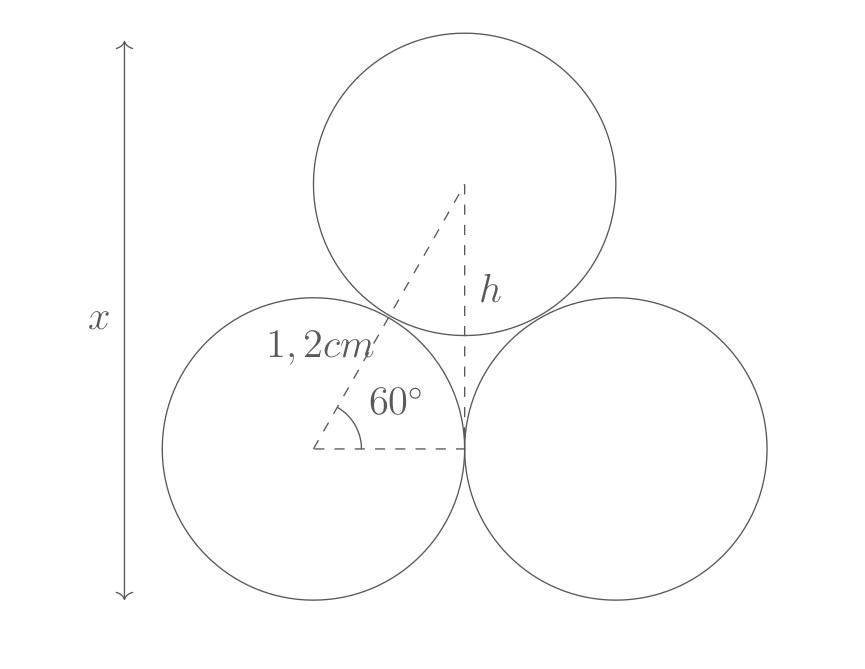
\includegraphics[width=\columnwidth,left]{../assets/geo.png}
        \end{column}
        \begin{column}{0.48\textwidth}
            \titlepage
        \end{column}
    \end{columns}

\end{frame}
}

%-------------------------------------------------------------------------------
% Sumário
%-------------------------------------------------------------------------------

\begin{frame}
    \frametitle{Sumário} % Table of contents slide, comment this block out to remove it
    \tableofcontents % Throughout your presentation, if you choose to use \section{} and \subsection{} commands, these will automatically be printed on this slide as an overview of your presentation
\end{frame}

%----------------------------------------------------------------------------------------
%	PRESENTATION SLIDES
%----------------------------------------------------------------------------------------
\section{Triângulos retângulos}
\subsection{Teorema de Pitágoras}
\begin{frame}[fragile]\frametitle{\subsecname}
O Teorema de Pitágoras é uma nova identidade presente nas dimensões do triângulo 
retângulo. Ela nos diz que:\\
\begin{alertblock}{}
    \textit{o quadrado do comprimento da hipotenusa é igual a soma dos 
    quadrados dos comprimentos dos catetos.}\\
\end{alertblock}
\begin{block}{Traduzindo para uma forma matemática temos então:}
    \begin{align*}
        a^2 &= b^2 + c^2
    \end{align*}
    Onde $a$ é o comprimento da hipotenusa, $b$ e $c$ o comprimento dos catetos.
\end{block}
\end{frame}
%------------------------------------------------

\begin{frame}[fragile]\frametitle{\subsecname}
    Dado o triângulo retângulo abaixo:
    \begin{figure}[H]
        \centering
        %\resizebox{\columnwidth}{!}{%
        \begin{tikzpicture}[scale=0.5\columnwidth/10cm]
            \coordinate (A) at (0,0);
            \coordinate (B) at (4,3);
            \coordinate (C) at (4,0);

            \tkzMarkRightAngle[size=.3](A,C,B);
            \draw (B)-- (C)-- (A)-- (B);
            \draw (A)-- node[above left] {$a$} (B); 
            \draw (B)-- node[right] {$c$} (C); 
            \draw (C)-- node[below] {$b$} (A); 
            % \draw (A)-- node[above left] {$4$} (B);
        \end{tikzpicture}
        %}
        % \caption{Triângulo retângulo $ABC$}
    \end{figure}
    O teorema nos diz que é possível obter o comprimento de 
    qualquer um dos lados, mesmo que os ângulos internos sejam desconhecidos, sendo 
    apenas necessário saber ao menos dois comprimentos desse triângulo.
\end{frame}

%------------------------------------------------

\begin{frame}[fragile]\frametitle{\subsecname}
    Em outras palavras, o teorema nos diz que a área em \textcolor{cyan}{ciano} é igual a soma das
    áreas \textcolor{blue!50}{azul} e \textcolor{red!50}{vermelho}.
    \begin{figure}[H]
        \centering
        %\resizebox{\columnwidth}{!}{%
        \begin{tikzpicture}[scale=0.5\columnwidth/10cm]
            \coordinate (A) at (0,0);
            \coordinate (B) at (4,3);
            \coordinate (C) at (4,0);
            \coordinate (D) at (7,3);
            \coordinate (E) at (7,0);
            \coordinate (F) at (0,-4);
            \coordinate (G) at (4,-4);
            \coordinate (H) at (-3,4);
            \coordinate (I) at (1,7);
            \draw[dashed, fill=blue!25] (B)--(D)--(E)--(C);
            \draw[dashed, fill=red!25] (A)--(F)--(G)--(C);
            \draw[dashed, fill=cyan!25] (A)--(H)--(I)--(B);

            \tkzMarkRightAngle[size=.3](A,C,B);
            \draw (B)-- (C)-- (A)-- (B);
            \draw (A)-- node[above left] {$a$} (B); 
            \draw (B)-- node[right] {$c$} (C); 
            \draw (C)-- node[below] {$b$} (A); 
            % \draw (A)-- node[above left] {$4$} (B);
        \end{tikzpicture}
        %}
        % \caption{Triângulo retângulo $ABC$}
    \end{figure}
\end{frame}
%------------------------------------------------

\subsection{Aplicações}
\begin{frame}[fragile]\frametitle{\subsecname}
    Um uso muito comum para o Teorema de Pitágoras é o cálculo da distância 
    entre dois pontos em um plano cartesiano.
    \begin{figure}[H]
        \centering
        \begin{tikzpicture}[scale=0.7\columnwidth/10cm]
            \begin{axis}[ymin=0,ymax=5,xmin=0,xmax=5]
                \addplot[mark=*] coordinates {(1,1)} node[above] {$(1,1)$};
                \addplot[mark=*] coordinates {(4,3)} node[above] {$(4,3)$};
                \draw(axis cs:1,1) -- node[above] {$a$} (axis cs:4,3);
                \draw[dashed] (axis cs:1,1) -- node[below] {$b$} (axis cs:4,1);
                \draw[dashed] (axis cs:4,1) -- node[right] {$c$} (axis cs:4,3);
            \end{axis}
        \end{tikzpicture}
    \end{figure}
\end{frame}

%------------------------------------------------

\begin{frame}[fragile]\frametitle{\subsecname}
    De modo geral, dado um ponto $P = (x_1,y_1)$ e um ponto $Q = (x_2,y_2)$ o 
    cateto $b$ tem comprimento $|x_2-x_1|$ e o cateto $c$ tem comprimento $|y_2-y_1|$
    \begin{figure}[H]
        \centering
        %\resizebox{\columnwidth}{!}{%
        \begin{tikzpicture}[scale=0.5\columnwidth/10cm]
            \coordinate (A) at (0,0);
            \coordinate (B) at (5,2);
            \coordinate (C) at (5,0);
            % \coordinate (D) at (0,3);
            \node[circle, fill, label={above:$(x_1,y_1)$}, inner sep=1.5pt] at (A) {};
            \node[circle, fill, label={above:$(x_2,y_2)$}, inner sep=1.5pt] at (B) {};
            % \node[circle, fill, label={left:$D$}, inner sep=2pt] at (D) {};
            % \draw[dashed] (A)--(D)--(B);
            \draw (A)-- node[above] {$a$} (B);
            \draw[dashed] (C)-- node[below] {$b$} (A);
            \draw[dashed] (B)-- node[right] {$c$} (C);
        \end{tikzpicture}
        %}
        % \caption{Triângulo retângulo $ABC$}
    \end{figure}
    Utilizando do teorema de Pitágoras onde $a^2 = b^2 + c^2$ temos que:
    \begin{align*}
        a^2 &= |x_2-x_1|^2 + |y_2-y_1|^2\\[1ex]
        a &= \sqrt{|x_2-x_1|^2 + |y_2-y_1|^2}
    \end{align*}
\end{frame}

%------------------------------------------------

\begin{frame}[fragile]\frametitle{\subsecname}

    \begin{block}{Distância entre pontos}
    Portanto a distância entre dois pontos quaisquer em um plano cartesiano 
    pode ser obtida através da fórmula:
    \begin{align*}
        a &= \sqrt{|x_2-x_1|^2 + |y_2-y_1|^2}
    \end{align*}
    \end{block}
\end{frame}

%------------------------------------------------

%------------------------------------------------

\begin{frame}
    \Huge{\centerline{Perguntas?}}
\end{frame}

%----------------------------------------------------------------------------------------

\end{document}